\chapter{State of the Art}
\label{chapter:state_of_the_art}

This chapter looks into previous work on collaborative robotics, action anticipation, and object recognition. \autoref{section:collaborative_robotics} covers the background concepts associated with collaborative robotics including communication methods and safety. \autoref{section:anticipation_system} explains the necessary fundamentals about action anticipation and provides some approaches from the current research direction in this theme. \autoref{section:object_recognition} explores the methods commonly used in object recognition.

\section{Collaborative Robotics}
\label{section:collaborative_robotics}

\acf{hrc} consists of robots and humans working in the same workspace towards a common goal. Classical industrial robots are usually automated to perform repetitive tasks that require high physical strength. On the other hand, tasks that require cognitive knowledge, flexibility, and precision are better suited for humans, even if they are physically weaker. \acs{hrc} aims to take advantage of both of their strengths and complement each others' weaknesses to increase manufacturing efficiency.

In a \acs{hrc} scenario, robots need to be different from the traditional ones, given that they will work in the same workspace as humans. According to \textcite{Castro2021}, \textquote{Collaborative robots need to be endowed with a set of abilities that enable them to act in close contact with humans, such as sensing, reasoning, and learning. In turn, the human must be placed at the center of a careful design where safety aspects and intuitive physical interaction need to be addressed as well.}. In \cite{CobotsWW}, it is stated that nowadays, collaborative robots are developed to be compact, easy to install and program, flexible, mobile, consistent, and precise. Additionally, they positively impact employees since they are responsible for monotonous and dangerous actions and reduce the production cost for the company.

\subsection{Human-Robot Communication}

Humans and robots can communicate through several methods, which can be direct such as using a console or a remote, or indirect, resulting from data captured from sensors. Based on \cite{Castro2021, Mukherjee2022, Semeraro2023}, the main methods for indirect communication can be seen in the diagram in \autoref{fig:hrc_data_sources} and can be described as follows:
\begin{figure}[ht]
    \centering
    %% by vsantos, 23 Mar 2023
\definecolor{vColorA}{HTML}{545454}
\definecolor{vColorB}{HTML}{8fa8d3}
\begin{tikzpicture}[scale=0.75,transform shape,
	mindmap,
	grow cyclic,
	every node/.append style={
				concept,
				inner sep=0pt,
				concept color=vColorB,
    font=\sffamily,
				}, %this is appended to all local props!
	concept color=vColorB,
	text=white,
%	font=\sffamily\bfseries\Large,
	level 1/.append style={
%							level distance=5cm,
%							sibling angle=60,
	%						font=\sffamily,
%							concept color=vColorB,
							},
	level 2/.append style={
%							level distance=2.75cm,
							sibling angle=45,
%							font=\small \sffamily,
							text=black,
%							concept color=white,
						  },
]

\node[] (HRC) at (0,0){\large\bfseries HUMAN ROBOT COMMUNICATION}
	[counterclockwise from = -30]
child[]
{
	node[](Gaze){GAZE}
	[clockwise from = 0]
	child{node[](dhp){Derived from human pose}}
	child{node[](eye) {Eye-tracking Wearable Device}}
}
child[]
{
	node [] (Semantics) {SEMANTICS}
	[counterclockwise from = 0]
	child{node[](hp){Human Poses}}
	child{node[](op) {Object Positions}}
}
child[]
{
	node [] (VoiceCommands) {VOICE COMMANDS}
}
child[]
{
	node []  (Gestures) {GESTURES}
		[counterclockwise from = 60] %[grow=180]
		child{node[](mv){Markerless Vision}}
		child{node[](vbm) {Vision based with Markers}}
		child{node[](di) {Depth Images}}
		child{node[](id) {Inertial Data}}	
		child{node[](pc) {Point clouds}}	
}
child[]
{
	node [] (Biometrics) {BIO-METRICS}
		[counterclockwise from = 180]
		child{node[](ma){Muscular Activity}}
		child{node[](ba) {Brain Activity}}	
}
child[]
{
	node [] (Emotions) {EMOTIONS}
}
;

\end{tikzpicture} 
    \caption{Common data sources in \acl{hrc}}
    \label{fig:hrc_data_sources}
\end{figure}
\begin{itemize}
\item \textbf{Gestures}: these are one of the main ways humans communicate, whether through simple movements or formal sign language. In the literature about \acs{hrc}, gestures can also commonly be found since they have the advantage of resisting ambient noise. Usually, gestures are captured with vision-based methods with either an RGB or RGB-D camera, so there is no need for unnatural movements. With vision, it is possible to include markers, but these may lead to occlusions and hinder the worker's movements. Consequently, there is also work in the literature that uses markerless vision to allow more unrestricted movements. Another way to capture the movements of the human worker would be to use wearable inertial sensors, which contain accelerometers and gyroscopes, but, once again, wearables can hinder the worker's movements. Finally, capturing point clouds using a LIDAR presents another possibility of capturing gestures without restricting the worker's motion.

% Do you mean spoken language by means of sound or written or typed text, or can it be more than this?

\item \textbf{Voice Commands}: talking is the most intuitive way for humans to communicate with each other. The advances in voice recognition and natural language processing make this a possible communication solution with robots. However, despite being intuitive, simple, effective, and even robust against lighting variations, when it comes to an industrial setting that contains significant sound noise, it becomes less valuable than the alternatives.

\item \textbf{Semantics}: semantic information about the objects can also help the global workflow. For example, suppose the robot is trained to recognize certain features in objects related to how it can pick them up. In this case, the robot can pick up a new object it has never seen before if it has a similar structure. Human actions can also be represented semantically by obtaining the poses of the human as a specific set of limbs, even if only partially. During action recognition, this can be used to know which objects the worker can interact with. Having semantic information about the pose of the human body also helps in the path-planning phase of the robot since it can use this information to avoid the worker and prevent collisions.

\item \textbf{Gaze}: this can be used to determine where the user's attention resides, giving a considerable amount of information that can trigger some action. There are two options to obtain the user's gaze. Wearable sensors can provide better results but are expensive and intrusive. On the other hand, algorithms that detect head pose and assume the gaze from it can also be used, which is a cheaper and non-intrusive solution.

\item \textbf{Emotions}: although this is a relatively new idea, some applications analyze the user's emotions from his facial expressions to have even more information in the algorithms.

\item \textbf{Biometrics}: \acf{emg} sensors can measure electrical signals generated by muscle contractions, while electroencephalography (EEG) signals are commonly used in brain-computer interfaces (BCIs). %\textcolor{blue}{And why not heart beat, breath, ...?}

\end{itemize}

\subsection{Safety}

Safety is one of the most critical topics in collaborative robotics and the first step toward establishing a collaborative environment. According to \cite{CobotsWW}, collaborative robots are able to safely work with people because they have sensitive sensors that can detect the human interrupting them, causing them to stop their actions, while traditional robots would potentially injure the worker. However, given that there are tasks that require the robot to move very close to the worker, some norms were implemented: ISO 10218-1 and 10218-2. From these two standards, \textcite{Castro2021} and \textcite{Villani2018} describe the four criteria from which at least one must be met:
\begin{enumerate}
  \item \textbf{Safety-rated monitored stop}: when a human enters the cobot's workspace, it completely stops.
  \item \textbf{Hand guiding}: when an operator manually moves the cobot, it is compliant.
  \item \textbf{Speed and separation monitoring}: as the human moves closer to the cobot, it becomes gradually slower.
  \item \textbf{Power and force limiting}: the cobot has its operation restricted in terms of force and torque.
\end{enumerate}

\begin{figure}[ht]
\captionsetup{width=0.8\textwidth}
\centerline{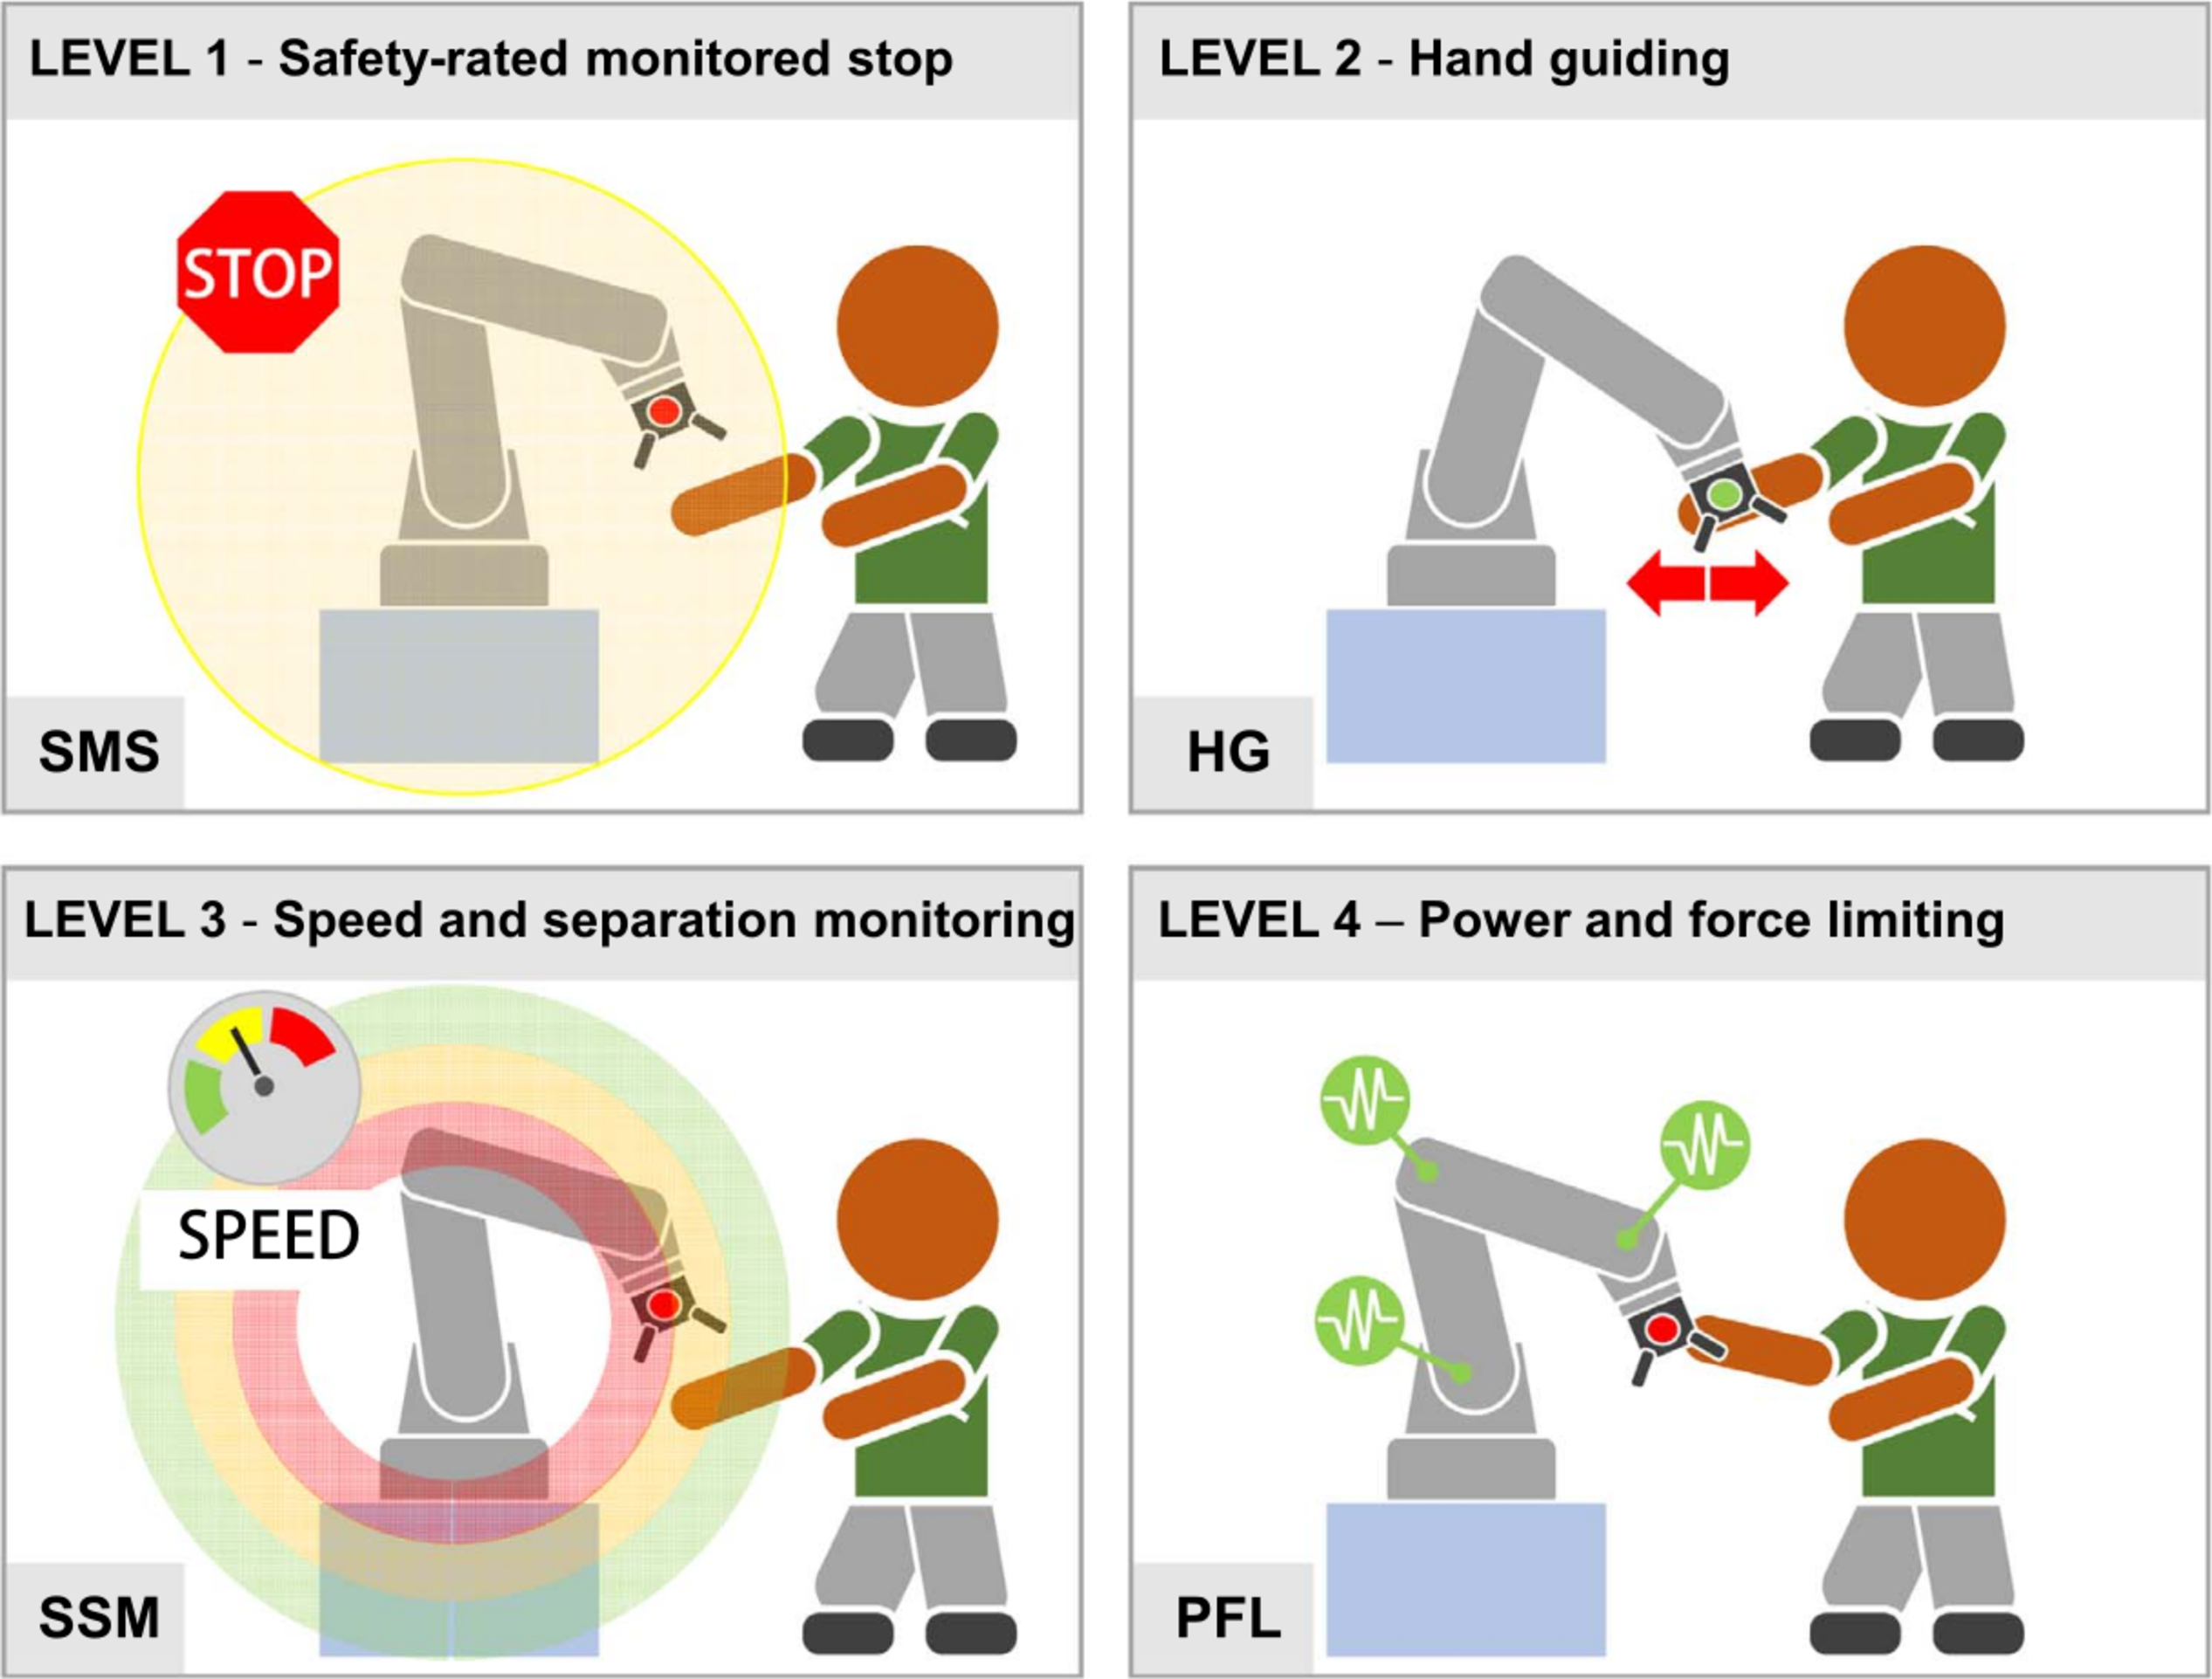
\includegraphics[width=0.8\textwidth]{figs/iso.pdf}}
\caption[The four collaborative operative modes identified by robot safety standards ISO modes 10218-1/2.]{The four collaborative operative modes identified by robot safety standards ISO modes 10218-1/2 \cite{Villani2018}.}
\label{fig:isonorms}
\end{figure}

\section{Anticipation System}
\label{section:anticipation_system}

\subsection{Concepts}

The concept of anticipation has been studied in several research fields and, in general, anticipation is viewed as the impact of predictions on the current behavior of a system, be it natural or artificial. A prediction model provides information about the possible future state of the environment and/or system. This perspective of looking to the future is related to the purpose of incorporating that information into a decision-making or planning process. Accordingly, the system becomes anticipatory when it incorporates such a model and, simultaneously, when it uses the model to change its current behavior.

Over the last few decades, experimental evidence of the existence of anticipatory biological processes at different levels of organization has been reported \cite{Deans2021,Poli2010}. The ability to modify behavior in anticipation of future events offers an adaptive advantage to living organisms with an impact on behavioral execution and learning. Anticipation is also considered one of the required abilities of cognitive robots operating in dynamically changing environments. The role of anticipation is to connect the robot’s action in the present to its final goal, helping the design of robots with an increased level of autonomy and robustness.

The fundamental aspects of anticipation lie at the intersection of concepts such as time and information, involving abilities such as perception and prediction. The above definition of anticipation contains a temporal element that provides a key division between anticipatory and non-anticipatory robots. Anticipatory robots make decisions based on current states and predicted future states using predictive models of the environment. At the other extreme of the spectrum are the robots that live in the present based on the current state of the observed environment, which are usually called reactive robots (e.g., the Braintenberg’s vehicles \cite{Braitenberg1986}). However, the behavior of a purely reactive robot is limited by its temporal horizon since they have no memory of the past to build a model of the world. Most of the current robots present a behavior influenced either by the current perception as well as by the memory of past perceptions but still lacking a perspective of the future.

Information provides another defining aspect of anticipation since the prediction of a future state depends on sensory data. The challenge arises from the moment that an anticipatory system operates based on a potential future state (even before it occurs) that can only be inferred from past and current information. The inherent uncertainty associated with the prediction process can be reduced through the acquisition of information, namely by using different sensory modalities. In this context, sensory fusion is a process often adopted to merge data from multiple sensors such that to reduce the amount of uncertainty that may be involved to produce more reliable knowledge about the future.

The nature of anticipation and the mechanisms that support it are considered open questions in \acs{ai} and robotics. Current research addresses fundamental questions such as: in which situations is anticipation useful? How can anticipatory processes be modeled and implemented in robotic systems? What are the impacts that may result from an anticipatory behavior? In the context of this dissertation proposal, anticipation is considered a combination of prediction and decision-making, as illustrated by the blocks diagram in \autoref{fig:anticipatorysystem}. The prediction model offers the possibility of incorporating action selection in their planning through a decision-making block, while the planning module relates to the robot’s actions. These modules can be developed separately, or an end-to-end learning technique could be used where the model learns the different parts from the perception to the feedback control. 

\begin{figure}[ht]
    \captionsetup{width=0.95\textwidth}
    \centering
    % Block of tikz code to draw the image of the Anticipatory System.
% Adapt at will.
% vsantos, 2023

\definecolor{colA}{HTML}{2a6099}
\definecolor{colB}{HTML}{729fcf}
\tikzset{
	myB/.style= %main block style
	{
		fill=colA,text=white, %comment this...
        %draw,  %...and uncomment this for a simpler diagram
		font=\sffamily,
		align=center,
		minimum height=1.5cm,
		text width=1.75cm,
		inner sep=2pt,
	},
	myT/.style= %the black triangle
	{
		isosceles triangle,
		fill=black,
		minimum height=8pt,
		isosceles triangle apex angle=140,
		anchor=apex,
        inner sep=1pt,
	},	
}

\def\nyDist{2.25cm}  %block separation
\pgfdeclarelayer{background layer}
\pgfsetlayers{background layer,main}
%Now the actual drawing
\begin{tikzpicture}[node distance=\nyDist]
\node [myB]              (per){Perception};
\node [myB,right of=per] (PM) {Prediction model};
\node [myB,right of=PM]  (DM) {Decision making};
\node [myB,right of=DM]  (MP) {Motion Planning};
\node [myB,right of=MP]  (FC) {Feedback Control};

\node [myB,below of=per] (per2) {Perception};
\node [myB, inner sep=0,
	fit={(PM) (MP)},
	yshift=-\nyDist,
	text depth=1.5em, %forced adjustment :-(
] (EEL) {End-to-end learning};
\node [myB,below of=FC] (FC2) {Feedback Control};

%Place all triangles with a loop ;-)
%Each triangle has a node name T1, T2, etc...
\foreach \NN [count=\i] in {PM,DM,MP,FC,EEL,FC2}
	\node [myT,at=(\NN.west)] (T\i) {};

%some tweaks to have the anticipatory layer well placed
\begin{pgfonlayer}{background layer}
\node [
	draw=colA,
	dotted,
	thick,
	fill=colB,
	fit=(PM.north west) (DM.south east),
	inner ysep=1em,
    yshift=0.5em,
	label={[anchor=north,font=\sffamily]north:Anticipatory layer}
	] (AL) {};
\end{pgfonlayer}

%Two auxiliary points to aid further
\coordinate (midL) at ($(per.west)!0.5!(per2.west)$);
\coordinate (midR) at ($(FC.east)!0.5!(FC2.east)$);

% The nodes at the extremes and the lines connecting them to the main blocks
\if{0}
\node [left of=midL,xshift=1cm,text width=1cm,font=\sffamily] (SI) {Sensor input};
\draw (SI) -- ([xshift=-10pt]midL) |- (per.west);
\draw (SI) -- ([xshift=-10pt]midL) |- (per2.west);

\node [right of=midR,xshift=-1cm,text width=1.25cm,font=\sffamily] (CO) {Control output};
\draw (CO) -- ([xshift=10pt]midR) |- (FC.east);
\draw (CO) -- ([xshift=10pt]midR) |- (FC2.east);
\fi

\node [left of=midL,xshift=1cm,text width=1cm,font=\sffamily] (SI) {Sensor input};
\draw (SI) |- (per.west);
\draw (SI) |- (per2.west);

\node [right of=midR,xshift=-1cm,text width=1.25cm,font=\sffamily] (CO) {Control output};
\draw (CO) |- (FC.east);
\draw (CO) |- (FC2.east);

\end{tikzpicture}
    \caption{Functional blocks of an anticipatory robotic system considering two alternative approaches: modules developed separately vs end-to-end learning.}
    \label{fig:anticipatorysystem}
\end{figure}

There are different situations in which an anticipatory response seems to be an essential ability for effective robot behavior. In an attempt to distinguish different types of anticipatory behaviors, three contexts in which a robot can operate are categorized below and the respective task requirements are presented as follows:
\begin{itemize}

\item \textbf{Time synchronization}: the interception of moving objects is central to several benchmark robotic tasks such as ball-catching and playing table tennis \cite{Carneiro2021, Wang2017}. These tasks are challenging due to the demanding spatial–temporal constraints, which require continuous coordination between visual, planning, and control systems. On the one hand, frequent repredictions of the target location are required as new observations become available. On the other hand, this progressive refinement imposes an online re-planning of robot motion such that the goal is achieved in time.

\item \textbf{Preventive safety}: systems that manage risk require some form of anticipatory mechanism such that the robot can adapt its behavior when an undesired situation occurs. Autonomous driving is an example of how predicting future events and reacting properly are important abilities to mitigate risk. Modeling behavior and predicting the future intentions of pedestrians are core elements to ensure that the driver stops the car safely or avoids the pedestrian in time.

\item \textbf{Coordinate joint activities in \acf{hri}}: humans have the ability to coordinate their actions when carrying out joint tasks with other partners \cite{Sebanz2006,Hoffman2007}. In the same line of thought, anticipation can enhance the ability of a robot to interact with a human partner by predicting their actions (or intentions) before selecting its own action plan. In collaborative contexts such as those that occur during manufacturing or assembly tasks, the main challenge is combining anticipation and planning in a context of high uncertainty due to the variability of human behavior in complex industrial environments. Anticipation seems to have a significant potential for more fluid and natural interaction with an impact on safety and cycle time.

\end{itemize}

\subsection{Approaches}

The ability of robots to accurately predict and anticipate human actions and intentions can greatly improve their ability to work safely and efficiently with humans in a shared workspace. Human intention recognition involves using sensors and machine learning algorithms to predict a human's intended action or task based on their movements, posture, and other contextual cues.

%The first step to anticipating the following action is to know which sensors should be used. Previously, several forms of communication between humans and robots were described. Still, these work in a more active way, and not all of them can be applied to action anticipation, where the user should not need to do anything for the robot to act. Essentially, there is a need to capture the human's body language or, in other words, his involuntary pose, gestures, and gaze, which became some of the most commonly used data to perform action anticipation.

Regarding the sensors used to capture the raw data, most literature suggests using a RGB camera. However, the captured images may be used in the following different ways:
\begin{itemize}
\item directly used as input to models which can extract features from the images;

\item used as input to frameworks that receive an image, process it, and return the keypoints, such as the skeleton joints of the person in the image; these keypoints can also then be used to assume the gaze of the human in the image such as in \textcite{Canuto2021} where the authors used OpenPose (explored in detail in \autoref{subsection:keypointdetection}) to obtain not only the skeleton joints but also the worker's gaze;

\item used to process the optical flow\cite{Gammulle2019, Wu2021, Rodriguez2019, Furnari2021};

\item if the human was wearing markers, the image can be used to obtain the positions of the markers obtaining gestures from the sequence of those positions \cite{Maeda2016};
\end{itemize}

Besides RGB cameras, some works, such as the one described in \textcite{Moutinho2023}, indicate the use of an RGB-D camera to capture both the color and the depth images, which contain the gestures and pose of the worker. Other than cameras, in \textcite{Tortora2019} IMU and \acs{emg} data was used as input to capture the gestures and anticipate the worker's action. When it comes to obtaining the worker's gaze, it is possible to do so from the RGB images as mentioned above, but it is also possible to use wearable sensors to capture it, such as in \textcite{Schydlo2018}.

% 1 modelo
% 2+ modelo
% modelo+decision making
% modelo+decision making+motion planning

After knowing which data is usually captured and provided to an algorithm, the remainder of this subsection explores possible algorithmic solutions present in previous work starting with those that are only about predicting the action of the human worker and then those that go a step further and reference how to go from a prediction to the action that the robot must execute as a response.

\subsubsection{Predictive Modeling Techniques}

In the state-of-the-art, anticipation is generally represented as a classification problem about predicting the next action of the worker, frequently done by using a sequence of images that must be classified as a particular future action class. Using \autoref{fig:superviseddiagram} as an example, the high-five action should be predicted before the frames that contain it are captured. The previous work with this kind of algorithm mainly includes \acfp{cnn} and \acfp{rnn}, with the latter being the most common.

\begin{figure}[ht]
    \centering
    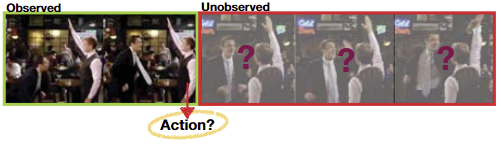
\includegraphics[width=0.95\textwidth]{figs/superviseddiagram.PNG}
    \caption[Action Anticipation using Supervised Learning diagram]{Action Anticipation using Supervised Learning diagram \cite{Gammulle2019}}
    \label{fig:superviseddiagram}
\end{figure}

% LSTM only examples
In \textcite{Furnari2021}, the authors aimed to predict the subsequent actions that someone wearing a camera would perform and the objects he would interact with. They used three datasets containing RBG frames from which they derived the optical flow and the objects in the environment. This data is then passed on to a Rolling-Unrolling \acf{lstm}. The Rolling \acs{lstm} (R-\acs{lstm}) is a network that continuously encodes the received observations and keeps an updated summary of the past. When it is time to make predictions about future actions, the Unrolling \acs{lstm} (U-\acs{lstm}) is used with its hidden and cell states equal to the current ones of the R-\acs{lstm}.

In \textcite{Schydlo2018}, the authors used an encoder-decoder recurrent neural network topology to predict human actions and intent where the encoder and the decoder are both \acs{lstm} networks. At each step, the decoder returns a discrete distribution of the possible actions making this algorithm able to consider multiple action sequences, which are then subject to a pruning method that reduces them to obtain the right action finally. In their work, these algorithms were tested in two different datasets, one containing RGB images with optical markers and gaze information from wearable sensors and another with RGB-D images.

% ResNet-34 + LSTM
In \textcite{Moutinho2023}, the authors aimed to increase the natural collaboration between the robot and the human in an assembly station by interpreting implicit communication cues. The data related to the environment was captured using an RGB-D camera. This data was then passed on to a ResNet-34, a pre-trained neural network that extracted the features from the images. These features are used as the input to a \acs{lstm} to perform human action anticipation.

% ResNet-50 + LSTM
In \textcite{Gammulle2019}, the authors aimed to predict future frames while at the same time predicting the following action. In their implementation, they used public datasets with videos from which they obtained RGB images and optical flow streams. To consider both data sources, they also used two ResNet-50's, which are pre-trained networks, one to get the input features from the image and another from the optical flow, and 2 \acs{lstm}s to take into account both sequences of inputs. Then the two results are merged into a final classification. They also used two Generative Adversarial Networks (GAN) to generate the subsequent frames, but this is different from the focus of the analysis.

%% VGG-16 + TTM
In \textcite{Wang2021}, the authors used video datasets to train a model that would predict a future action from the observed frames. They used three pre-trained neural networks in their work: VGG-16, TS, and ConvNet, to extract features from the images. Then these features were aggregated using a Temporal Transformer Module (TTM), and finally, a Progressive Prediction Module (PPM) would anticipate the worker's future action. This article also addresses the issue of specifying what the algorithm should consider as an action. Although most of the literature often implies that the last frames captured by the camera are considered an action, given that those are the frames that contain the last action made by the user, the authors of this article go into greater detail. They tested and evaluated how many frames should be considered as the last action to obtain the best results using a metric from \textcite{Geest2016} named per-frame calibrated average precision (cAP) calculated with \eqref{eq}. In \cite{Wang2021} it is defined with
\begin{equation}
cAP=\frac{\sum_k cPrec(k) \times I(k)}{P},
\label{eq}
\end{equation}
\textquote{... where calibrated precision $cPrec=\frac{TP}{TP+FP/w}$, $I(k)$ is an indicator function that is equal to 1 if the cut-off frame $k$ is a true positive, $P$ denotes the total number of true positives, and $w$ is the ratio between negative and positive frames. The mean $cAP$ over all classes is reported for final performance.}.

%% CNN
In \textcite{Rodriguez2019}, the authors aimed to predict the next action by first predicting the following motion images. They used datasets containing videos and then processed them to obtain motion images. These motion images become the input of a convolutional autoencoder network that generates the following motion images. These images are then passed to a \acs{cnn} that processes them and makes action predictions for the future. The final action prediction is obtained from the results of the previous network and those of a second \acs{cnn}, which analyzes the original RGB images.

%% architecture with TSN
In \textcite{Wu2021}, the author's goal was to predict the following action someone wearing a camera would perform after some time. Initially, the optical flow was obtained from the captured images, and both were used as input to the model. The model is comprised of a Temporal Segment Network (TSN), a \acs{cnn}, and a \acs{lstm} to predict the future frame features and then use them to perform the required classification.

\subsubsection{From Prediction to Planning}

After predicting the next action of the worker, the robot must execute some action as a response to complete the anticipation process. This subsubsection contains articles that go beyond the predictive model and have relevant details for the integration of the model in a controller.

In \textcite{Canuto2021}, the authors aimed to predict the following action using a \acs{lstm}. In their work, they used a dataset captured with an RGB camera. From these images, they obtained the objects in the environment, the human skeleton joints extracted over time using OpenPose, and the gaze derived from the joints. Then the three data sources were given to the \acs{lstm} as input to perform the desired classification. In this process, the authors use an adaptive threshold on the uncertainty of the recurrent neural network, which makes the model need a certain level of certainty to classify the action as a particular class. This creates a more robust solution since a standard supervised learning algorithm would predict the class with the highest probability even if the model has low certainty about every category.

% Look-up table
In \textcite{Maeda2016}, the authors aimed to reduce the delay in the robot's response by anticipating the human worker and providing a screw or a plate accordingly. They captured the environment using an RGB camera and tracked the hand using optical markers. Then they predicted the following human action using a look-up table containing different orders for assembly actions. With the nearest neighbor algorithm, the actions of the human would be matched with a particular order. The limitation of this method is that all possible sequences need to be on the table because if they are not there, then the robot will match with a different order which may be undesirable. If the robot eventually notices that it did the wrong action, it would then follow a hard-coded contingency trajectory to return to the pre-grasping position. When performing a handover action, the previously captured data is used to generate possible trajectories and this is given to the feedback controller as a reference.

% LSTM + CNN
In \textcite{Zhang2022}, the authors aimed to predict the intention of the human worker to provide him with the required piece. To achieve this, they used an RGB camera to capture the data from the environment. Then the images are given to a convLSTM framework where the \acs{cnn} part is in charge of extracting features from the input images, and these features are then passed on to the \acs{lstm} to predict the intention. This article also tackles the issue of having several possible assembly orders. It solves it by creating a phase at the beginning of the collaboration in which the robot learns the assembly actions and their order from a demonstration. After the prediction of the intention of the worker, the robot proceeds to fetch the required piece. It uses a \acs{cnn} to recognize said piece and \acs{ros} \acf{ompl} to handle the trajectory planning jobs. In terms of safety, the authors defined speed limits for the robot and ensured that the robot would avoid the workspace of the human. Then when it needs to move closer to the user, its speed is reduced to guarantee the user's safety.

In \textcite{Huang2016}, the authors' goal is to make the robot use the anticipated actions of the worker to decide its tasks. It monitors the worker's gaze using a wearable device and uses it to predict his intent using a \acf{svm}. After predicting it, the robot uses an anticipatory motion planner named \textquote{MoveIt!} to plan its motion according to a certain confidence threshold. This means that while it is unsure of what the human wants, the robot starts to move toward the item it thinks the user wants but only really moves completely when it surpasses the threshold.

\section{Object Recognition}
\label{section:object_recognition}

The idea underlying this study is to explore the possibility of establishing a relationship between the object grasped by the human operator and his current needs in collaborative scenarios. The immediate conceptual roots can be traced to the Activity Theory \cite{Kuutti1996} whose main concept is "activity" defined as a purposeful and developing interaction between actors ("subjects") and the world ("objects"). This framework has established itself as a key concept for research in \acf{hci} and interaction design.

This section provides an overview of existing literature and research relevant to this study. In particular, the recognition of the object grasped by the user is the central block when it comes to achieving the main purpose. It is organized into two subsections – "object sensing" and "hand sensing" – to help categorize and differentiate methods that primarily focus on capturing and analyzing data related to the object itself from those that explicitly use data from the human hand to infer the object being grasped. 

\subsection{Object Sensing}
Approaches within the "object sensing" category leverage visual information extracted from images or videos of the objects the user is interacting with, by using techniques from computer vision and machine learning to discern object identities based on their visual attributes. A common approach involves the extraction of visual features that can encompass color histograms, texture descriptors, contour shapes, and local key-points. Early works in this domain \cite{Taubin1992,Mindru1999,Sarfraz2006} applied traditional image processing techniques to extract features such as shape moments and color histograms, leading to initial success in recognizing simple objects. The surge of progress seen in recent years is largely due to the latest developments in deep learning \cite{Wu2020}, particularly \acs{cnn}s, and geometric reasoning \cite{Barabanau2020}.

Deep learning has had an enormous impact on perception tasks with the design of effective architectures for real-time object recognition, providing significant advancements in accuracy and robustness. \acs{cnn}s have demonstrated remarkable performance in extracting hierarchical features from images \cite{Ren2017}. Transfer learning, where pre-trained models are fine-tuned for specific tasks, has enabled efficient object recognition even with limited training data \cite{Zhuang2021}. A relevant vision-based approach is the one in which the process of recognizing the human-grasped object, across consecutive frames, comprises two sub-processes: hand tracking and object recognition. The hand detection and tracking system is commonly used for defining a bounding box around the grasped object that describes its spatial location. This initial step can, in turn, simplify the object recognition algorithm as it can focus attention solely on the region where the object is likely to be present. This reduces the search space and the required computational resources. Object detection frameworks like YOLO (You Only Look Once) and Faster R-\acs{cnn} fall under this category. They divide the RGB image into a grid and predict bounding boxes and class probabilities directly from the grid.  

In parallel to deep learning, the recent availability of inexpensive RGB-D sensors has enabled significant improvements in scene modeling and human pose estimation. Some studies explore the fusion of multiple modalities to enhance object recognition. These approaches combine visual information with other sensory data, such as depth information from 3D sensors \cite{Zimmermann2018,Rato2022}. This integration of modalities has shown promise in improving recognition accuracy, especially in scenarios with varying lighting conditions or occlusions. Researchers have also studied how to leverage information from multiple viewpoints (i.e., multi-view 3D object recognition) to enhance recognition accuracy \cite{Qi2021}. This approach is particularly relevant for 3D objects, where recognizing an object's 3D structure from different viewpoints can aid in robust recognition. Techniques like using 3D point clouds, multi-view \acs{cnn}s, or methods that combine RGB images and depth information fall under this category.

Despite their successes, methods within the "Object Sensing" category are often constrained by the variability of object appearances, limited viewpoint coverage, and sensitivity to illumination changes. As a result, the focus on object characteristics alone may not provide a complete solution, particularly in situations where the human hand's interaction with the object plays a crucial role.

\subsection{Hand Sensing}
Recognizing objects based on the interactions of the human hand is a complex problem due to the intricate nature of \acfp{hoi} and the variability in grasp patterns and gestures \cite{Chao2018,Gkioxari2018,Cao2021,Liu2021}. Achieving accurate and real-time recognition involves understanding the relationships and dynamics between a human hand and the objects it interacts with (e.g., the interaction context, the person's actions, and the patterns that emerge over time), as well as the tactile and kinesthetic feedback generated during manipulation. Additionally, variations in grasp styles, object sizes, and orientation further worsen the complexity of the task. Several works propose interaction reasoning networks for modeling spatio-temporal relationships between hands and objects in egocentric videos during activities of daily life, such as playing an instrument, kicking a ball, opening a drawer (one-handed interaction), opening a bottle (two-handed interaction, cutting a vegetable with a knife). Main advances are due to the development of several human-centric datasets (e.g., V-COCO \cite{Gupta2015}, HICO-DET \cite{Chao2018} and HCVRD \cite{Zhuang2018}) that annotate the bounding boxes of each human actor, the object with which he/she is interacting and the corresponding interaction. However, the creation of large-scale, diverse, and annotated datasets was still an ongoing effort.

Some works consider the \acs{hoi} as a manifestation of human intention or purpose of action \cite{Koppula2015,Hayes2017,Furnari2019,Xu2019,Roy2021}. Despite the growing need for detection and inference of \acs{hoi}s in practical applications, such as collaborative robotics, the problem of recognizing objects based on hand-object interactions is inherently complex. Instead of addressing the full complexity of \acs{hoi} recognition, several works have adopted targeted approaches that address specific aspects of the problem without necessarily delving into the entire spectrum of interactions. A recent work investigated the influence of physical properties of objects such as shape, size, and weight on forearm electromyography (\acs{emg}) signals and the opportunities that this sensing technology brings in hand-object interaction recognition and/or for object-based activity tracking \cite{Fan2018}. Despite the relevance of the work, it is difficult to apply in collaborative assembly scenarios given the complexity of the required setup that requires sensor attachment, calibration, and training. Some other limitations may include user-dependent variability, muscle fatigue and discomfort, and/or interference from other electrical devices.   

Another line of research, closest to this work, focuses on tracking the positions of hand and finger landmarks during interactions. By monitoring the spatial relationships of these landmarks, these methods aim to deduce the object's identity based on the specific manipulations applied. This approach captures critical information about the hand's interaction without necessarily modeling the full complexity of interactions. A glove-based interaction approach has been proposed by Paulson et al. \cite{Paulson2011} in the \acs{hci} domain to investigate a grasp-based selection of objects in office settings. Authors showed that hand posture information solely can be used to recognize various activities in an office, such as dialing a number, holding a mug, typing at the keyboard, or handling the mouse. The classification of hand posture is performed using the nearest-neighbor algorithm.  In a similar work based on a data glove, Vatavu et al. \cite{Vatavu2013} proposed the automatic recognition of the size and shape of objects using the posture of the hand during prehension. The objects used in the experiments consisted of six basic shapes (cube, parallelepiped, cylinder, sphere, pyramid, and a thin plate) and, for each shape, three different sizes (small, medium, and large). Twelve right-handed participants took part in the experiments using a 5DT Data Glove Ultra equipped with 14 optical sensors. These sensors are distributed as follows: 10 sensors measure finger flexion (two sensors per finger) and four sensors measure abduction between fingers.

The study compared several classifiers derived from the nearest-neighbor approach with a \acf{mlp} and a multi-class \acs{svm}. The best results were achieved with the $K$-nearest-neighbor classification approach when combining the results of individual postures across an entire time window of half a second. The experiments carried out included the capture of hand postures when grasping and maintaining a stable grip for reliable translation of the objects. The results showed that object size and shape can be recognized with up to \SI{98}{\percent} accuracy when using user-specific metrics. The authors also pointed out the lower accuracy for user-independent training and the variability of individual grasping postures during object exploration. Although in general, the proposed approach recognizes the physical properties of the grasped objects with high accuracy, wearing a glove directly on the hand is intrusive and troublesome, interfering with the natural movement of the fingers.

When attempting to model human grasping, researchers have focused their attention on defining a comprehensive taxonomy of human grasp types \cite{Feix2015} and the multifaceted factors that influence the choice of grasping, including user intentions \cite{Mackenzie1994}, object properties \cite{Feix2014}, and environmental constraints \cite{Puhlmann2016}. \textcite{Mackenzie1994} theorize the existence of a cognitive model that converts the object’s geometry properties and user’s intent into a motor program driving the hand and finger motions. From this seminal work, several studies on human reach-to-grasp actions have consistently shown that the natural kinematics of prehension allows for predicting the object he/she is going to grasp, as well as the subsequent actions that will be carried out with that object. \textcite{Feix2014} provided an analysis of human grasping behaviors showing the correlation between the properties of the objects and the grasp choice. More recently, the works of \textcite{Betti2018} and \textcite{Egmose2018} focus on the reach-to-grasp phase. Their finding shows that grasp formation is highly correlated with the size and shape of the object to be grasped, as well as strongly related to the intended action. These insights promise improved interaction by exploring the ability in which the robot can predict the object the user intends to grasp or to recognize the one he/she is already holding, provided that the hand kinematics information is extracted and processed in real-time.

In line with this, \textcite{Valkov2023} investigated the feasibility and accuracy of recognizing objects based on hand kinematics and \acs{lstm} networks. The data is extracted from a Polhemus Viper16 electromagnetic tracking system with 12 sensors attached to the hand and fingers. On the one hand, the study focuses on the size discrimination of 9 synthetic objects: three regular solids (sphere, box, and cylinder) in three different sizes (small – \SI{2}{cm}, medium – \SI{4}{cm} and large – \SI{6}{cm}).  On the other hand, a different set of seven objects (pen, glue, bottle, Rubik’s cube, volcano-egg, toy, and scissors) was used for object discrimination. The data recorded during the experiments includes a phase in which participants were asked to reach and grasp the object starting from a fixed initial position. The results demonstrated that \acs{lstm} networks can predict the time point at which the user grasps an object with \SI{23}{ms} precision and the current distance to it with a precision better than \SI{1}{cm}. Furthermore, the size and the object discrimination during the reach-to-grasp actions were achieved successfully with accuracy above \SI{90}{\percent} using $K$-fold cross-validation. Although the results are still preliminary, the leave-one-out cross-validation showed a significant degradation in the performance of the models compared to the $K$-fold validation. While the tracking system offers many advantages, there are also practical limitations such as sensor attachment and comfort, line-of-sight requirements, interference and noise, and calibration and drift. 

